\documentclass{article}
\usepackage{comment}
\usepackage[table]{xcolor}
\usepackage[polish]{babel}
\addto\captionspolish{\renewcommand{\figurename}{Ilustracja}}
\usepackage[utf8]{inputenc}
\usepackage[T1]{fontenc}
\usepackage[a4paper,top=2cm,bottom=2cm,left=3cm,right=3cm,marginparwidth=1.75cm]{geometry}
\usepackage{amsmath}
\usepackage{graphicx}
\usepackage[colorlinks=true, allcolors=violet]{hyperref}
\usepackage{blindtext}
\usepackage{algorithmicx}
\usepackage[style=polish]{csquotes}
\usepackage{float}
\usepackage{subcaption}
\usepackage{multirow}
\usepackage{gensymb}
\usepackage{siunitx}
\usepackage[
  separate-uncertainty = true,
  multi-part-units = repeat
]{siunitx}
\usepackage{array}
\usepackage{algpseudocode}
\usepackage{xcolor}
\newtheorem{lemma}{Lemat}
\newtheorem{theorem}{Twierdzenie}

\usepackage{algorithm}
\usepackage{booktabs}

\begin{document}
\begin{titlepage}
    \centering
    {\fontsize{60}{30}\selectfont \textbf{Metody Sztucznej Inteligencji 2} \par}
    \vspace{1.5cm}
    {\fontsize{30}{20}\selectfont Projekt 2 -- raport końcowy \par}
    \vspace{5cm}
    {\fontsize{36}{20}\selectfont \textbf{Zastosowanie algorytmu Monte Carlo Tree Search w grze w unikanie ciasnych bliźniaków} \par}
    \vspace{7.5cm}

    {\fontsize{26}{20}\selectfont
    Yahor Kachanouski\\
    Miłosz Wysocki
    \par}
    \vspace{0.5cm}
    \vfill

    {\large czerwiec 2026 \par}
\end{titlepage}

\tableofcontents
\newpage

% --------------------------------------------------------------------------------------------
\section{Streszczenie}

W ramach projektu zaimplementowano i przebadano rodzinę algorytmów z grupy
Monte Carlo Tree Search (MCTS) zastosowanych do asymetrycznej, dwuosobowej gry
w unikanie ciasnych bliźniaków. Gra polega na sekwencyjnym budowaniu słowa
nad ustalonym alfabetem~$\Sigma$ aż do osiągnięcia maksymalnej długości~$L$:
gracz \emph{wskazujący} (Pointer) wybiera pozycję wstawienia, a gracz
\emph{wstawiający} (Inserter) określa literę. Zwycięża ten, kto zmusi
przeciwnika do utworzenia podciągu postaci $xx$ (ciasnego bliźniaka),
albo doprowadzi słowo do długości~$L$ bez takiego podciągu.

Zaimplementowano modułowy framework MCTS, w którym fazy
\emph{selekcji}, \emph{symulacji} i \emph{propagacji wstecznej} są wymiennymi
strategiami. Porównano klasyczny algorytm UCT~\cite{Kocsis2006}, wariant
UCB1-Tuned~\cite{Auer2002}, MCTS-Solver z propagacją udowodnionych
węzłów~\cite{Winands2008} oraz dwie heurystyki dziedzinowe -- filtrującą
symulację i Progressive Bias~\cite{Chaslot2008}.

Kluczowy eksperyment to dwuwymiarowa siatka konfiguracji
$|\Sigma|\in\{3,\dots,10\}\times L\in\{5,\dots,40\}$, dla każdej z nich
przeprowadzono po~20 partii (1000 iteracji MCTS na ruch). Wyniki potwierdzają
hipotezę o wpływie parametrów gry: krótkie słowa i duży alfabet faworyzują
Insertera, długie słowa i mały alfabet -- Pointera. Gdy spojrzeć na
zsumowany odsetek wygranych z obu ról, klasyczny UCT i wariant UCB1-Tuned
osiągają w naszej grze praktycznie identyczne wyniki ($\approx 50\%$ \mbox{vs}
$50\%$); spodziewana przewaga UCB1-Tuned nie ujawniła się. Heurystyka
filtrująca symulację okazała się natomiast najsilniejszą badaną
modyfikacją -- agregat zwycięstw wynosi $\approx 64\%$ wobec $\approx 36\%$
dla klasycznego UCT. Wariant MCTS-Solver wbrew oczekiwaniom zachowuje się
gorzej od klasycznego UCT (sumarycznie $\approx 42\%$ wobec $\approx 58\%$),
przy czym regresja koncentruje się w roli Insertera. W raporcie omawiamy
prawdopodobne przyczyny tej regresji oraz sugerujemy ich
implementacyjne, a nie algorytmiczne, źródło.
\newpage

% --------------------------------------------------------------------------------------------
\section{Gra w unikanie ciasnych bliźniaków}

Gra w unikanie ciasnych bliźniaków to wymyślona, asymetryczna gra turowa
oparta na klasycznym problemie kombinatoryki słów -- unikaniu powtórzeń
typu \emph{kwadrat}, badanym już przez Thuego na początku XX wieku
\cite{Thue1906,Lothaire2002}. Z perspektywy teorii gier jest to gra
dwuosobowa o sumie zerowej, z pełną informacją i bez elementów losowych:
każdy kolejny stan planszy wynika w stu procentach z deterministycznych
decyzji podjętych przez graczy w poprzednich turach. Te własności czynią
grę naturalnym poligonem doświadczalnym dla algorytmów MCTS.

\subsection{Definicje formalne}
Aby precyzyjnie opisać zasady, definiujemy podstawowe pojęcia:
\begin{itemize}
    \item \textbf{Alfabet ($\Sigma$)} -- z góry ustalony, skończony zbiór
    znaków (np.~$\Sigma=\{a,b,c\}$).
    \item \textbf{Słowo ($w$)} -- ciąg znaków zbudowany z liter alfabetu;
    gra rozpoczyna się od słowa pustego~$\epsilon$.
    \item \textbf{Bliźniaki} -- dwa identyczne, rozłączne podciągi w obrębie
    jednego słowa.
    \item \textbf{Ciasne bliźniaki (kwadraty)} -- szczególny przypadek
    bliźniaków tworzących spójne podsłowo postaci $xx$, gdzie $x$ jest
    dowolnym niepustym ciągiem znaków (np.~\textit{aa}, \textit{baba},
    \textit{abcabc}).
\end{itemize}

\subsection{Zasady gry i role graczy}
Rozgrywka jest parametryzowana przez dwa czynniki: używany alfabet~$\Sigma$
oraz maksymalną dozwoloną długość słowa~$L$. Gracze wykonują tury
naprzemiennie, ich role i dostępne akcje są jednak całkowicie asymetryczne.

\begin{itemize}
    \item \textbf{Gracz~1 (Wskazujący / Pointer):} W swojej turze analizuje
    aktualne słowo~$w$ o długości~$N$ i wskazuje pozycję (indeks od~$0$
    do~$N$), na której ma pojawić się nowa litera. Celem Pointera jest
    wymuszenie na przeciwniku stworzenia ciasnych bliźniaków.
    \item \textbf{Gracz~2 (Wstawiający / Inserter):} W swojej turze wybiera
    jedną z liter alfabetu~$\Sigma$ i wstawia ją na pozycję narzuconą przez
    Pointera. Celem Insertera jest budowanie słowa tak, aby uniknąć
    ciasnych bliźniaków aż do osiągnięcia limitu~$L$.
\end{itemize}

Gra kończy się w jednym z dwóch przypadków:
\begin{enumerate}
    \item W słowie pojawiają się ciasne bliźniaki -- zwycięstwo Pointera.
    \item Słowo osiąga długość~$L$ i nie zawiera ciasnych bliźniaków --
    zwycięstwo Insertera.
\end{enumerate}
Gra nie przewiduje remisów.

\subsection{Przykład rozgrywki}
Poniżej zaprezentowano krótki przykład partii z alfabetem
$\Sigma=\{a,b,c\}$ i limitem $L=5$. Początkowy stan to słowo puste,
kursor wstawiania oznaczono symbolem~$|$.

\begin{enumerate}
    \item \textbf{Tura~1:} Pointer wskazuje jedyną dostępną pozycję
    (indeks~0). Inserter wstawia literę~\textit{a}. Aktualne słowo:
    \textbf{a}.
    \item \textbf{Tura~2:} Pointer wskazuje pozycję na końcu (indeks~1:
    $a|$). Inserter wstawia literę~\textit{b}. Aktualne słowo: \textbf{ab}.
    \item \textbf{Tura~3:} Pointer wskazuje pozycję w środku (indeks~1,
    między \textit{a} i \textit{b}: $a|b$). Inserter wstawia
    literę~\textit{c}. Aktualne słowo: \textbf{acb}.
    \item \textbf{Tura~4:} Pointer wskazuje pozycję na samym końcu (indeks~3:
    $acb|$). Inserter decyduje się wstawić literę~\textit{b}. Aktualne
    słowo: \textbf{acbb}.
\end{enumerate}

Po czwartej turze system weryfikujący stan gry wykrywa, że na końcu słowa
powstały ciasne bliźniaki (podsłowo \textit{bb}). Gra kończy się
natychmiastowym zwycięstwem Pointera, przed osiągnięciem limitu znaków~$L$.
Zła decyzja Insertera w czwartej turze (wstawienie \textit{b} zamiast
\textit{a} lub \textit{c}) doprowadziła do jego porażki.

\subsection{Algorytm detekcji ciasnych bliźniaków}

Kluczowym składnikiem silnika gry jest algorytm wykrywający wystąpienie
ciasnych bliźniaków. Ogólny problem wyszukiwania powtórzeń w słowie jest
rozstrzygalny w czasie wielomianowym; istnieją algorytmy o złożoności
$\mathcal{O}(n\log n)$ wykorzystujące zaawansowane struktury danych
\cite{Lothaire2002}. Ponieważ w naszej grze maksymalna długość słowa nie
przekracza kilkudziesięciu liter, narzut stałej związany z budową takich
struktur danych przewyższa ich asymptotyczne korzyści.

Zaimplementowano zoptymalizowany algorytm typu \textit{brute-force}
z lokalną detekcją, opisany w pseudokodzie poniżej. Wykorzystuje on dwa
spostrzeżenia:
\begin{enumerate}
    \item długość pojedynczego bliźniaka jest co najwyżej połową długości
    słowa,
    \item po wstawieniu pojedynczej litery nowe ciasne bliźniaki mogą
    powstać wyłącznie w okienkach zahaczających o wstawiony znak.
    Wystarczy zatem sprawdzić $\mathcal{O}(n)$ takich okienek zamiast
    $\mathcal{O}(n^2)$.
\end{enumerate}

\begin{algorithm}[H]
\caption{Lokalna detekcja ciasnych bliźniaków}
\begin{algorithmic}[1]
\Function{CzyPowstalBlizniak}{$slowo, indeks\_nowego\_znaku$}
    \State $N \gets \text{długość}(slowo)$
    \For{$L \gets 1$ \textbf{to} $\lfloor N / 2 \rfloor$}
        \State $dlugosc\_blizniaka \gets 2 \times L$
        \State $start\_min \gets \max(0, indeks\_nowego\_znaku - dlugosc\_blizniaka + 1)$
        \State $start\_max \gets \min(indeks\_nowego\_znaku, N - dlugosc\_blizniaka)$
        \For{$poczatek \gets start\_min$ \textbf{to} $start\_max$}
            \State $lewa\_polowa \gets slowo[poczatek \dots poczatek + L - 1]$
            \State $prawa\_polowa \gets slowo[poczatek + L \dots poczatek + 2L - 1]$
            \If{$lewa\_polowa = prawa\_polowa$}
                \State \Return \textbf{Prawda}
            \EndIf
        \EndFor
    \EndFor
    \State \Return \textbf{Fałsz}
\EndFunction
\end{algorithmic}
\end{algorithm}

% --------------------------------------------------------------------------------------------
\section{Metoda Monte Carlo Tree Search (MCTS)}

\subsection{Historia}

Algorytmy z rodziny Monte Carlo Tree Search (MCTS) są obecnie jednym
z najważniejszych paradygmatów w sztucznej inteligencji dla gier o dużej
złożoności stanów. Termin \emph{Monte Carlo Tree Search} po raz pierwszy
został wprowadzony w pracy Couloma w 2006 roku, który zastosował go do
programu grającego w Go~\cite{Coulom2006}. W tym samym roku Kocsis
i Szepesvári opublikowali kluczową pracę wprowadzającą algorytm UCT,
stanowiący fundament współczesnych implementacji MCTS~\cite{Kocsis2006}.

Przełom nastąpił w 2016 roku, gdy program AlphaGo firmy DeepMind pokonał
mistrza świata w Go, Lee Sedola. Sukces ten był wynikiem połączenia
przeszukiwania drzewa MCTS z głębokimi sieciami neuronowymi do oceny
stanów~\cite{Silver2016}. Od tego momentu MCTS stanowi złoty standard
w grach z pełną informacją.

\subsection{Architektura i fazy algorytmu MCTS}

Jak wskazuje obszerny przegląd metod MCTS Browne i in.~\cite{Browne2012},
siła tego algorytmu opiera się na budowaniu asymetrycznego drzewa
przeszukiwań poprzez wielokrotne powtarzanie czterofazowej pętli.
Pozwala to skupić zasoby obliczeniowe na najbardziej obiecujących
gałęziach drzewa.

W trakcie przebiegu gry ustalona liczba iteracji jest wykonywana przed
każdym ruchem algorytmu. Algorytm buduje drzewo podczas całej rozgrywki;
każda iteracja składa się z czterech kroków:

\begin{enumerate}
    \item \textbf{Selekcja} -- algorytm rozpoczyna od korzenia drzewa
    (aktualnego stanu gry) i rekurencyjnie wybiera węzły potomne aż do
    dotarcia do węzła, który nie został w pełni wyekspandowany.
    \item \textbf{Ekspansja} -- po dotarciu do węzła rozszerzalnego, do
    drzewa dodawany jest jeden nowy węzeł potomny, reprezentujący kolejny,
    niezbadany jeszcze legalny ruch z danego stanu.
    \item \textbf{Symulacja} -- z nowo utworzonego węzła przeprowadzana jest
    szybka symulacja rozgrywki aż do osiągnięcia stanu końcowego.
    \item \textbf{Propagacja wsteczna} -- wynik symulacji jest propagowany
    w górę ścieżki, aż do korzenia. W każdym odwiedzonym węźle aktualizowane
    są statystyki: liczba odwiedzin oraz liczba zwycięstw.
\end{enumerate}

\subsection{Adaptacja MCTS do gry w ciasnych bliźniaków}

Środowisko gry spełnia założenia gry dwuosobowej z pełną informacją
o sumie zerowej, jednak jego asymetryczny charakter (różne akcje
w turach Pointera i Insertera) wymaga drobnej adaptacji algorytmu:

\begin{itemize}
    \item \textbf{Węzły drzewa} reprezentują stany gry. Każdy poziom drzewa
    na przemian opisuje stan po wskazaniu indeksu przez Pointera oraz stan
    po wstawieniu litery przez Insertera.
    \item \textbf{Selekcja i propagacja} -- gracze realizują przeciwstawne
    cele, dlatego wynik propagowany w fazie backpropagacji jest
    interpretowany z perspektywy gracza wykonującego ruch w danym węźle.
    Identycznie wzory selekcji (UCT, UCB1-Tuned) są obliczane z punktu
    widzenia aktualnego movera.
    \item \textbf{Ekspansja} -- ze względu na szybki przyrost liczby
    dozwolonych ruchów (wzrost długości słowa zwiększa liczbę dostępnych
    indeksów dla Pointera), MCTS dodaje jedynie po jednym nowym wariancie
    ruchu na iterację.
    \item \textbf{Symulacja} -- domyślna faza rozgrywki polega na losowym
    przeplataniu wyboru indeksów i wstawiania liter, dopóki algorytm
    detekcji bliźniaków nie zaraportuje ich obecności albo słowo nie
    osiągnie maksymalnej długości.
\end{itemize}

% --------------------------------------------------------------------------------------------
\section{Algorytm UCT (Upper Confidence Bound applied to Trees)}

\subsection{Dylemat eksploracji i eksploatacji}
Głównym wyzwaniem w fazie selekcji jest tzw. dylemat eksploracji
i eksploatacji. Algorytm musi decydować, czy podążać ścieżkami, które do
tej pory przynosiły najlepsze rezultaty (eksploatacja), czy też badać
węzły rzadko odwiedzane, które mogą ukrywać jeszcze lepsze rozwiązania
(eksploracja). Rozwiązaniem tego problemu jest metoda \textbf{UCT},
wprowadzona przez Kocsisa i Szepesváriego~\cite{Kocsis2006}, adaptująca
strategię UCB1 z problemów wielorękich bandytów do drzew decyzyjnych.

\subsection{Formuła matematyczna}
W trakcie selekcji, dla każdego w pełni wyekspandowanego węzła, algorytm
oblicza wartość UCT dla wszystkich jego dzieci i wybiera to, które
maksymalizuje:

\begin{equation}
UCT_i = \bar{X}_i + C \sqrt{\frac{\ln N}{N_i}}
\end{equation}

gdzie $\bar{X}_i = W_i/N_i$ to \textbf{eksploatacja} (średni odsetek
wygranych węzła~$i$), $N_i$ -- liczba odwiedzin węzła~$i$, $N$ -- liczba
odwiedzin rodzica, a $C$ -- stała eksploracji (zwykle $\sqrt{2}$).
W ramach naszego projektu wartość $\bar{X}_i$ jest zawsze obliczana
z perspektywy gracza aktualnie wykonującego ruch w danym węźle, zgodnie
z konwencją gier o sumie zerowej.

% --------------------------------------------------------------------------------------------
\section{Zaimplementowane modyfikacje algorytmu}

W projekcie zaimplementowano dwie modyfikacje fazy obliczania wagi węzła
oraz dwie heurystyki dziedzinowe. Wszystkie warianty są wymienne -- każdy
gracz może niezależnie zestawić swój algorytm z dowolnej kombinacji
strategii selekcji, symulacji i propagacji wstecznej.

\subsection{MCTS-Solver (propagacja udowodnionych węzłów)}
Algorytm \emph{Monte-Carlo Tree Search Solver}~\cite{Winands2008} jest
modyfikacją klasycznego MCTS, szczególnie użyteczną w grach typu
\emph{nagła śmierć} (\textit{sudden-death}), do których należy gra
w unikanie ciasnych bliźniaków. Standardowy MCTS nie potrafi rozpoznać
zagwarantowanych węzłów końcowych na etapie selekcji, ponieważ opiera
się wyłącznie na wartościach uśrednionych. MCTS-Solver rozwiązuje ten
problem, dodając do węzłów flagę \emph{stanu udowodnionego}.

Logika propagacji jest następująca:
\begin{itemize}
    \item Jeżeli ruch prowadzi do terminalnego stanu, węzeł jest natychmiast
    oznaczany odpowiednim statusem (proven win lub proven loss z perspektywy
    movera).
    \item Jeżeli wszystkie dzieci węzła mają status proven loss z perspektywy
    movera, węzeł rodzica otrzymuje status proven loss.
    \item Jeżeli choć jedno dziecko ma status proven win z perspektywy
    movera, rodzic otrzymuje status proven win.
\end{itemize}

W zaimplementowanym wariancie, gdy w fazie selekcji jakieś dziecko ma
status proven win dla aktualnego movera, jest wybierane deterministycznie
(omijając formułę UCT).

\subsection{UCB1-Tuned}
Klasyczna formuła UCB1 uzależnia czynnik eksploracji wyłącznie od liczby
odwiedzin danego węzła, ignorując stabilność jego dotychczasowych wyników.
Heurystyka \textbf{UCB1-Tuned}~\cite{Auer2002} rozszerza oryginalny wzór
o szacowaną wariancję wyników z przeprowadzonych symulacji.

W naszej grze, z uwagi na brak remisów, każda symulacja przyjmuje wartość
binarną (sukces lub porażka), co odpowiada rozkładowi Bernoulliego.
Wariancja takiego rozkładu wynosi $V=p(1-p)$, gdzie $p$ to empiryczny
odsetek wygranych z danego węzła. Wprowadzenie elementu $p(1-p)$ sprawia,
że MCTS dynamicznie redukuje poziom eksploracji dla węzłów o pewnym
wyniku ($p\approx 0$ lub $p\approx 1$, gdzie wariancja dąży do zera) oraz
przekierowuje moc obliczeniową na dogłębne badanie węzłów niestabilnych
($p\approx 0{,}5$, gdzie wariancja osiąga maksimum).

Całkowita waga węzła~$i$ w UCB1-Tuned wynosi:
\begin{equation}
    Score_i = \bar{X}_i + \sqrt{\frac{\ln N}{n_i} \min\left(\frac{1}{4}, V_i(N)\right)}
\end{equation}
gdzie górna granica oszacowanej wariancji jest dana wzorem:
\begin{equation}
    V_i(N) = \hat{\sigma}_i^2 + \sqrt{\frac{2 \ln N}{n_i}}
\end{equation}
($\hat{\sigma}_i^2$ -- wariancja empiryczna, drugi składnik koryguje
skutek małej liczby odwiedzin).

\subsection{Heurystyka w fazie symulacji}
Najprostszym sposobem na implementację wiedzy dziedzinowej są tzw.
\emph{symulacje wzbogacone}~\cite{Chaslot2008}, w których zastępuje się
całkowicie losowe rollouty filtrami deterministycznymi. W naszej
implementacji symulacja heurystyczna stosuje reguły:
\begin{itemize}
    \item \textbf{Inserter}: zamiast wybierać literę w pełni losowo,
    skrypt symulacyjny odrzuca litery, które natychmiast tworzą ciasnego
    bliźniaka. Jeżeli każda litera prowadzi do bliźniaka, gracz jest
    zmuszony do ruchu przegrywającego.
    \item \textbf{Pointer}: jeżeli istnieje pozycja, w której Inserter --
    niezależnie od wybranej litery -- musi utworzyć bliźniaka, Pointer
    deterministycznie wybiera tę pozycję.
\end{itemize}

\subsection{Progressive Bias}
Drugim miejscem na wdrożenie heurystyki jest faza selekcji, poprzez metodę
\emph{Progressive Bias}~\cite{Chaslot2008}. Polega ona na dodaniu do wagi
węzła składnika wynikającego z heurystycznej oceny ruchu:
\begin{equation}
    Score'_i = Score_i + \frac{w \cdot H(i)}{n_i + 1}
\end{equation}
gdzie $w$ to waga heurystyki, $H(i)$ -- jej wartość, a dzielenie przez
$n_i + 1$ sprawia, że wpływ heurystyki maleje wraz z liczbą odwiedzin.

W naszej implementacji $H$ definiuje:
\begin{itemize}
    \item dla Insertera: bezpieczeństwo litery, mierzone jako $1$ minus
    jej częstość występowania w okolicy kursora,
    \item dla Pointera: niebezpieczeństwo wskazywanej pozycji, mierzone
    jako udział liter alfabetu, których wstawienie utworzy bliźniaka.
\end{itemize}
Progressive Bias jest zaimplementowany jako dekorator dowolnej strategii
selekcji, dzięki czemu można go łączyć zarówno z UCT, jak i UCB1-Tuned.

% --------------------------------------------------------------------------------------------
\section{Implementacja}

Projekt został napisany w języku \textbf{Python~3.10+} z naciskiem na
modułową, kompozycyjną architekturę. Algorytm MCTS rozbito na trzy
niezależne strategie -- selekcję, symulację i propagację wsteczną --
zgodnie ze wzorcem projektowym \emph{Strategy}. Dzięki temu każdy gracz AI
może być skonfigurowany jako dowolna kombinacja tych elementów, a dodanie
nowego wariantu wymaga jedynie napisania nowej klasy implementującej
odpowiedni interfejs (np.\ \texttt{SelectionStrategy}).

Najważniejsze elementy infrastruktury projektu:
\begin{itemize}
    \item silnik gry oddzielony od logiki AI (moduł \texttt{src.engine}),
    \item węzły i orkiestrator MCTS (\texttt{src.mcts}) działające na
    abstrakcyjnym interfejsie silnika gry,
    \item interfejs graficzny w \textbf{PyQt6} (\texttt{src.ui})
    udostępniający tryby Człowiek--AI oraz AI--AI z możliwością obserwacji
    rozgrywki, a także wyboru poziomu trudności (regulowanego liczbą
    iteracji MCTS na ruch),
    \item bezgłowy (\textit{headless}) runner eksperymentów konfigurowany
    plikami \textbf{YAML} (\texttt{src.run\_match}). Pojedynczy plik
    konfiguracji może definiować wiele meczów, których wyniki są zapisywane
    do plików CSV i następnie agregowane.
\end{itemize}

Wykorzystane biblioteki ograniczono do niezbędnego minimum: \texttt{numpy}
(generowanie ziaren losowości), \texttt{PyQt6} (GUI), \texttt{pyyaml}
(wczytywanie plików konfiguracyjnych) oraz \texttt{tqdm} (pasek postępu
podczas dłuższych serii eksperymentów). Wykresy heatmap zaprezentowane
w niniejszym raporcie wygenerowano w skryptach pomocniczych z użyciem
\texttt{pandas}, \texttt{matplotlib} i \texttt{seaborn}.

Ważnym szczegółem konwencji rozgrywki w runnerze eksperymentów jest fakt,
że pierwszy ruch Pointera (przy słowie pustym jest tylko jedna możliwa
pozycja: indeks~0) jest wymuszony. Decyzja ta usuwa trywialny ,,wybór'',
który nie niósłby żadnej informacji algorytmicznej, i ujednolica warunki
porównania między wariantami algorytmu.

% --------------------------------------------------------------------------------------------
\section{Hipotezy badawcze}

W ramach badań porównywano skuteczność wariantów MCTS oraz własności samej
gry. Hipotezy postawione przed pracą eksperymentalną zachowano
w niezmienionej formie:

\subsection*{Hipoteza H1}
\paragraph{H1:} Wariant UCB1-Tuned osiągnie wyższy odsetek wygranych
w grze przeciwko klasycznemu wariantowi UCT.

\subsection*{Hipoteza H2A}
\paragraph{H2A:} Wariant MCTS-Solver osiągnie wyższy odsetek wygranych
w grze przeciwko klasycznemu wariantowi UCT.

\subsection*{Hipoteza H2B}
\paragraph{H2B:} Wariant MCTS-Solver nie wykaże znaczącej przewagi nad
klasycznym UCT przy niskiej liczbie iteracji i dużym rozmiarze drzewa.

\subsection*{Hipoteza H3}
\paragraph{H3:} Zastosowanie heurystyk poprawi skuteczność algorytmu.

\subsection*{Hipoteza H4}
\paragraph{H4:} Balans szans na zwycięstwo graczy zależy od długości
słowa i rozmiaru alfabetu. Inserter ma tym większe szanse, im większy
jest alfabet; przy długim słowie i krótkim alfabecie większe szanse ma
Pointer.

% --------------------------------------------------------------------------------------------
\section{Plan eksperymentów}

W celu sprawdzenia powyższych hipotez przeprowadzono serię turniejów
w trybie AI--AI, w których badane warianty algorytmów grały przeciw sobie
w obu rolach. Wszystkie eksperymenty wykonano z użyciem identycznej liczby
iteracji MCTS (1000 na ruch) i stałej eksploracji $C=\sqrt{2}$, co
odpowiada wartościom standardowym w literaturze.

Każdy mecz dla ustalonej pary wariantów oraz ustalonych parametrów gry
($|\Sigma|, L$) składał się z 20 partii rozegranych z różnymi ziarnami
RNG (\texttt{base\_seed}=42). Dla badania całej przestrzeni gry przyjęto
siatkę:
\begin{itemize}
    \item rozmiar alfabetu $|\Sigma|\in\{3,4,5,6,7,8,9,10\}$,
    \item maksymalna długość słowa $L\in\{5,10,15,20,25,30,35,40\}$.
\end{itemize}
Daje to 64 konfiguracje dla pojedynczej pary wariantów. W niniejszym
raporcie dyskutowanych jest pięć zestawień: trzy badane warianty
(UCB1-Tuned, MCTS-Solver oraz heurystyczna symulacja) zestawione
z klasycznym UCT, przy czym dla UCB1-Tuned i MCTS-Solver przebadano obie
role. Łącznie odpowiada to $5\times 64\times 20 = 6400$ rozegranym
partiom.

Klasyczny UCT (oznaczany \emph{Classic}) traktowany jest jako odniesienie
i zestawiany z każdym z pozostałych wariantów. Pomiary wykonano w obu
rolach: raz badany wariant gra jako Pointer (Classic jest Inserterem),
raz jako Inserter (Classic jest Pointerem). Zabieg ten pozwala oddzielić
efekt samego algorytmu od efektów asymetrii ról.

Wszystkie konfiguracje turniejów zapisano w plikach YAML; wyniki każdej
partii (m.in.\ zwycięzca, liczba ruchów, końcowe słowo, czas rozgrywki)
zostały zapisane w plikach CSV i przekształcone w heatmapy prezentowane
w następnej sekcji.

% --------------------------------------------------------------------------------------------
\section{Wyniki eksperymentów}

Poniżej prezentujemy pięć map cieplnych obrazujących \textbf{odsetek
wygranych Pointera} dla pięciu różnych par wariantów algorytmu.
Zielony kolor oznacza przewagę Pointera, czerwony -- przewagę Insertera.
Granica ($\approx 50\%$, kolor żółty) wyznacza strefy, w których oba
warianty osiągają zbliżone wyniki.

\subsection{Wpływ parametrów gry -- weryfikacja H4}

Pierwsze obserwacje dotyczą samej gry, niezależnie od wariantu algorytmu.
Wszystkie pięć heatmap pokazuje ten sam ogólny wzorzec:
\begin{itemize}
    \item \textbf{lewy dolny trójkąt} (długie słowa, mały alfabet) jest
    głęboko zielony -- Pointer wygrywa praktycznie 100\% partii. Inserter
    nie ma dostatecznej liczby liter, by uniknąć powtórzeń;
    \item \textbf{prawy górny trójkąt} (krótkie słowa, duży alfabet) jest
    głęboko czerwony -- Inserter wygrywa praktycznie 100\% partii. Duży
    alfabet daje swobodę wyboru bezpiecznej litery, a krótki limit nie
    zdąży wymusić bliźniaka;
    \item \textbf{pas środkowy} (przekątna gridu) zawiera strefy
    wyrównane, w których przewagi nad przeciwnikiem żaden wariant nie
    uzyskuje całkowicie.
\end{itemize}

Wynik ten w pełni potwierdza hipotezę \textbf{H4}: balans gry zależy
bezpośrednio od stosunku $L$ do $|\Sigma|$. Z punktu widzenia projektanta
turniejów oznacza to, że różnice między wariantami algorytmu najwyraźniej
ujawniają się w strefie wyrównania -- w skrajnych obszarach gry sytuacja
jest na tyle przesądzona, że jakość selekcji ma niewielkie znaczenie.

\subsection{UCB1-Tuned vs.~klasyczny UCT -- weryfikacja H1}

\begin{figure}[H]
\centering
\begin{subfigure}[b]{0.48\textwidth}
    \centering
    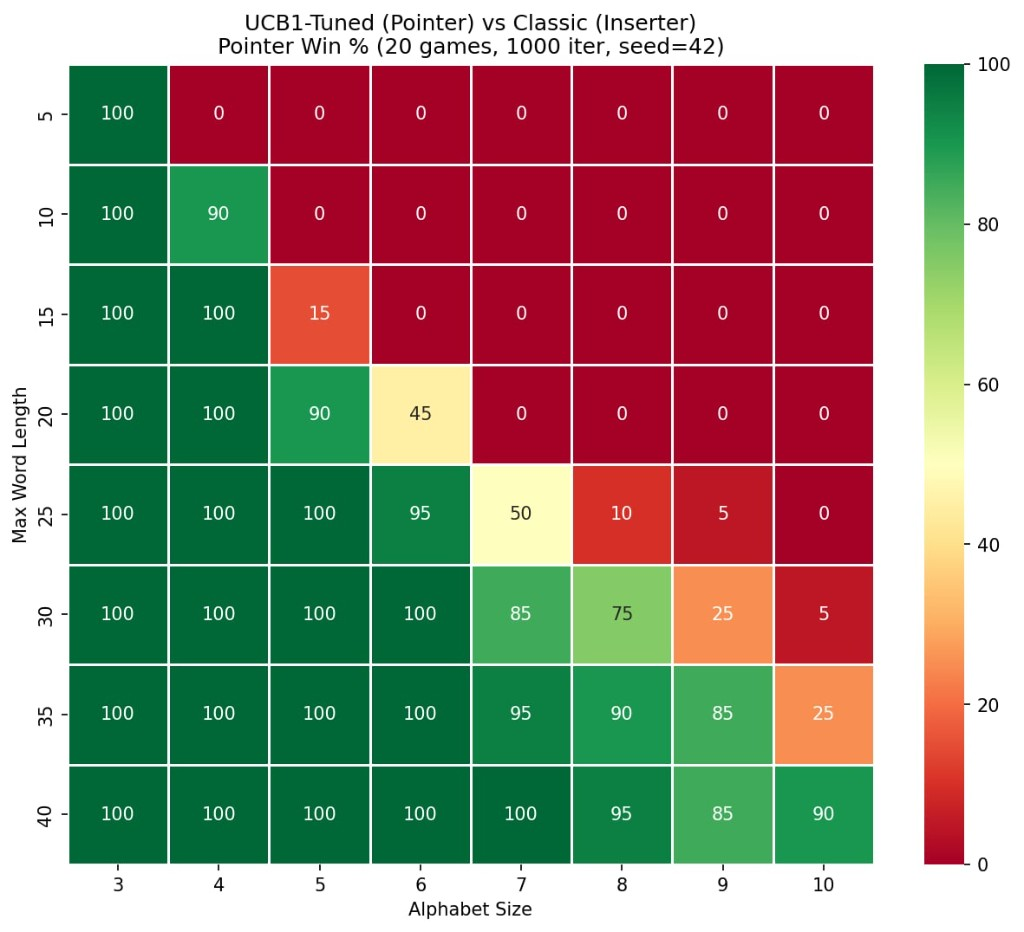
\includegraphics[width=\textwidth]{figures/hm_ucb1tuned_vs_classic.png}
    \caption{UCB1-Tuned w roli Pointera}
\end{subfigure}
\hfill
\begin{subfigure}[b]{0.48\textwidth}
    \centering
    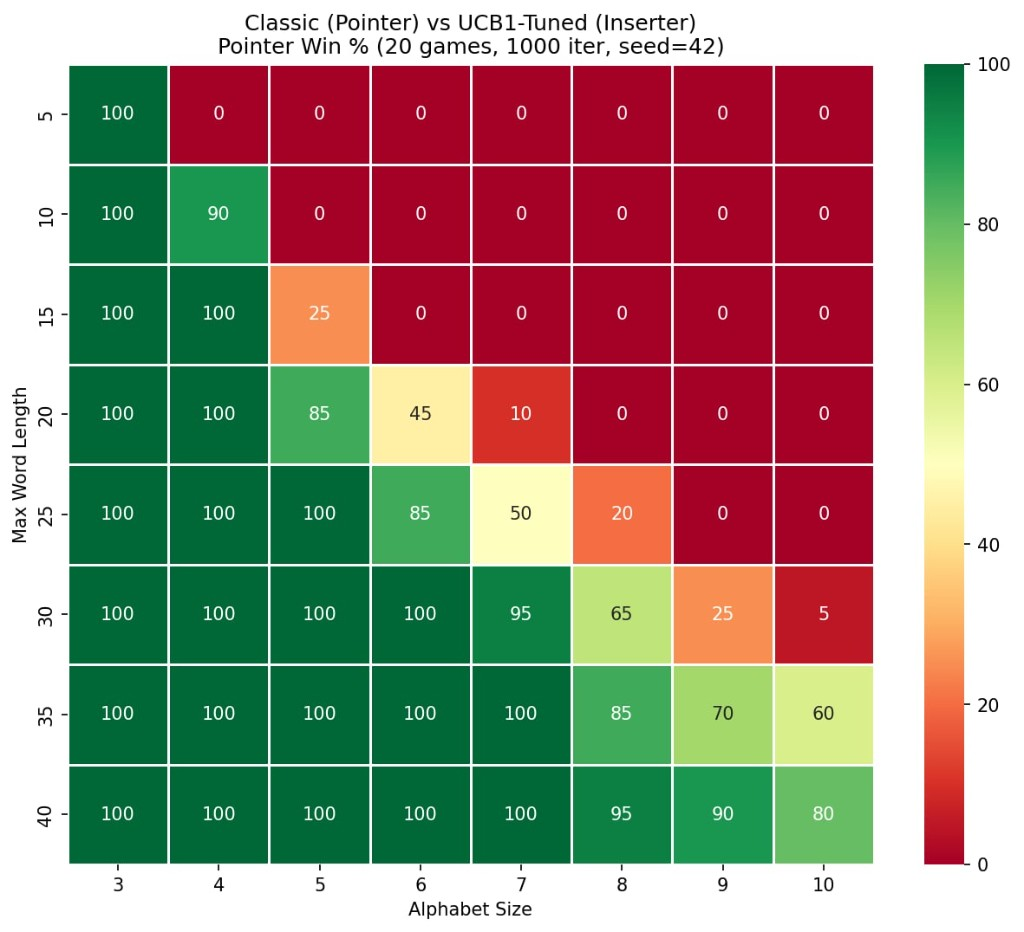
\includegraphics[width=\textwidth]{figures/hm_classic_vs_ucb1tuned.png}
    \caption{UCB1-Tuned w roli Insertera (komplement do wartości podanej
    w mapie)}
\end{subfigure}
\caption{Konfrontacja UCB1-Tuned z klasycznym UCT.}
\label{fig:ucb1tuned}
\end{figure}

Wzrokowe porównanie obu heatmap sugeruje na pierwszy rzut oka, że są one
niemal nieodróżnialne -- przewaga Pointera w ,,domenie Pointera'' oraz
Insertera w ,,domenie Insertera'' jest praktycznie identyczna. Aby
oszacować różnicę ilościowo, zsumowano odsetki wygranych Pointera
w każdej z 64 komórek siatki. Wartości te traktujemy jako przybliżony,
zagregowany ,,wynik turnieju'' obejmujący wszystkich $64\times 20=1280$
partii reprezentowanych przez heatmapę:

\begin{table}[H]
\centering
\begin{tabular}{lrr}
\toprule
Heatmapa & Suma punktów Pointera & Średni odsetek \\
\midrule
UCB1-Tuned (Pointer) vs Classic (Inserter) & 3355 & 52,4\% \\
Classic (Pointer) vs UCB1-Tuned (Inserter) & 3380 & 52,8\% \\
\bottomrule
\end{tabular}
\end{table}

Po przeniesieniu wyników UCB1-Tuned z roli Insertera ,,na drugą stronę''
otrzymujemy łączny wynik UCB1-Tuned w obu rolach na poziomie
$\approx 49{,}8\%$ wygranych, podczas gdy klasyczny UCT osiąga
$\approx 50{,}2\%$. Różnica $0{,}4$ punktu procentowego mieści się
w naturalnym szumie przy 2560 partiach. \textbf{Hipoteza H1 nie znajduje
więc potwierdzenia} -- w naszej grze formuła UCB1-Tuned nie różni się
od klasycznego UCT w żadnym praktycznie istotnym stopniu.

Brak efektu nie zaskakuje aż tak bardzo, jak mogłoby się wydawać. Dynamika
gry w ciasne bliźniaki jest silnie binarna: w środkowych etapach partii
węzły mają zazwyczaj odsetek wygranych albo bliski $0$, albo bliski $1$
(albo trafiamy na pole, w którym Inserter musi się szybko poddać, albo
mamy bezpieczne kontynuacje). Wariancja $V=p(1-p)$ jest wówczas również
bliska zeru, więc dodatkowy człon UCB1-Tuned przestaje cokolwiek korygować
względem klasycznego UCB1.

\subsection{Heurystyka symulacji vs.~klasyczny UCT -- weryfikacja H3}

\begin{figure}[H]
\centering
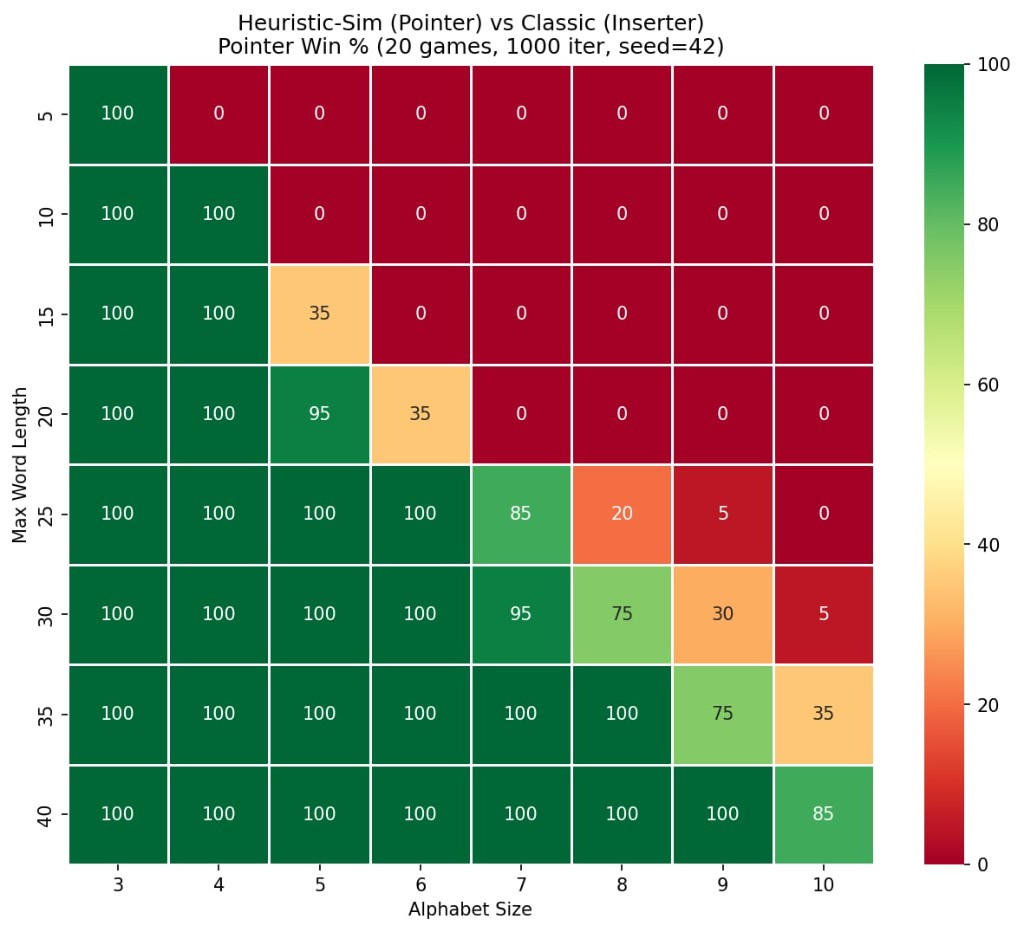
\includegraphics[width=0.75\textwidth]{figures/hm_heuristic_vs_classic.png}
\caption{Symulacja heurystyczna w roli Pointera przeciw klasycznemu UCT
w roli Insertera.}
\label{fig:heuristic}
\end{figure}

W tym układzie Pointer korzysta z symulacji wzbogaconej -- filtrującej
litery niebezpieczne dla Insertera oraz wymuszającej deterministyczny
wybór pozycji o gwarantowanej wygranej. Heatmapa pokazuje wyraźnie
poszerzony ,,zielony trójkąt'' wygranych Pointera kosztem strefy
wyrównania.

Ilościowo: zagregowany odsetek wygranych heurystycznego Pointera wynosi
$54{,}3\%$ (suma punktów $3475$), a wynik analogicznego eksperymentu
w odwróconych rolach (heurystyczny Inserter przeciwko klasycznemu
Pointerowi) daje $75{,}3\%$ wygranych Insertera. Po zsumowaniu obu ról
heurystyczna symulacja osiąga $\approx 64\%$ wygranych przeciwko
klasycznemu UCT, czyli przewagę rzędu $14$ punktów procentowych.
\textbf{Hipoteza H3 potwierdza się więc jednoznacznie.}

Warto podkreślić, że zysk z heurystycznej symulacji jest niemal o rząd
wielkości większy niż z wymiany formuły selekcji (UCB1-Tuned), mimo iż
jest to jedna z prostszych modyfikacji do zaimplementowania. W grach
o silnie nieliniowej dynamice końcowej (jednoruchowa porażka) jakość
rolloutu odgrywa kluczową rolę: filtr heurystyczny eliminuje całkowicie
,,nierealistyczne'' przebiegi, w których losowy Inserter sam wbija się
w bliźniaka pomimo posiadania bezpiecznych ruchów.

\subsection{MCTS-Solver vs.~klasyczny UCT -- weryfikacja H2A i H2B}

Rolom MCTS-Solver poświęcamy odrębne wykresy.

\begin{figure}[H]
\centering
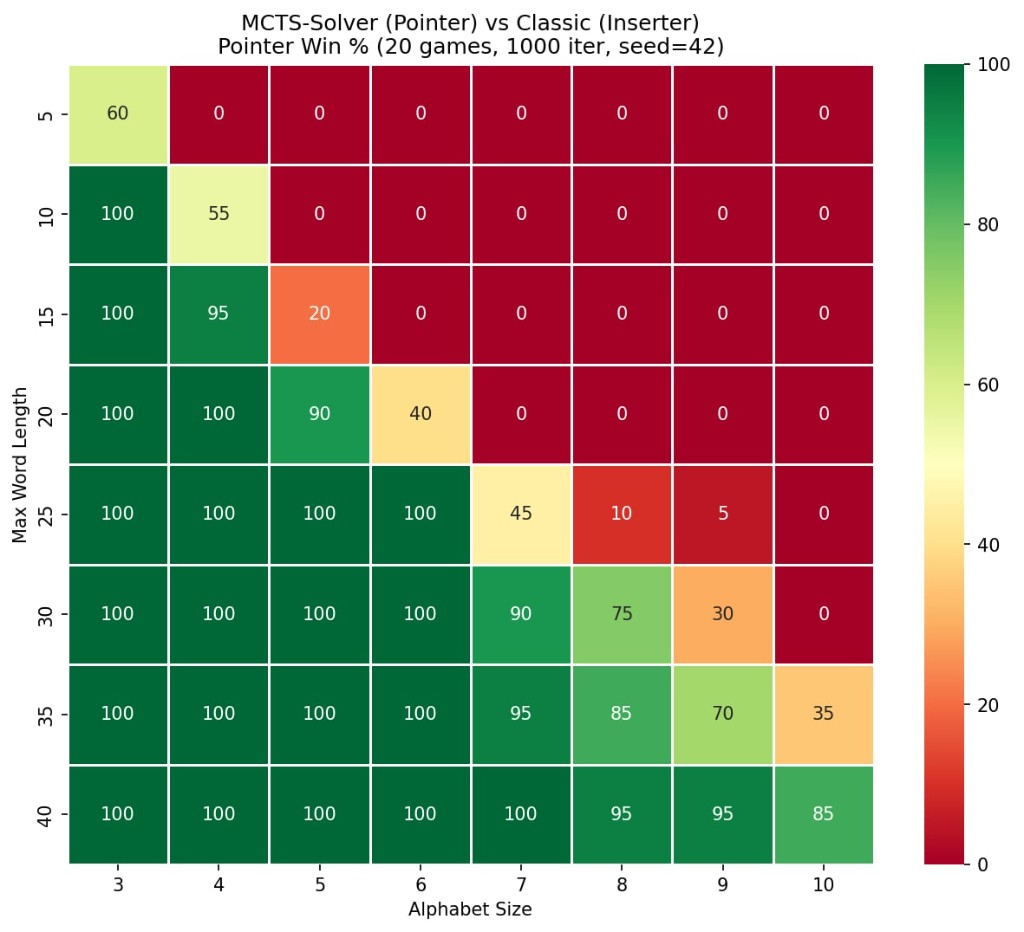
\includegraphics[width=0.75\textwidth]{figures/hm_solver_vs_classic.png}
\caption{MCTS-Solver w roli Pointera przeciw klasycznemu UCT w roli
Insertera.}
\label{fig:solver_pointer}
\end{figure}

W roli Pointera MCTS-Solver radzi sobie podobnie do pozostałych
wariantów -- jego zagregowany odsetek wygranych wynosi $51{,}2\%$
(dla porównania UCB1-Tuned $52{,}4\%$). W pozycjach, w których Pointer
ma szansę na ,,krótki'' dowód wygranej (często wystarczy 1--2 ruchy do
wymuszenia bliźniaka), propagacja flag udowodnionych mogłaby teoretycznie
przynieść istotny zysk; w naszych danych takiej przewagi nie widać.

\begin{figure}[H]
\centering
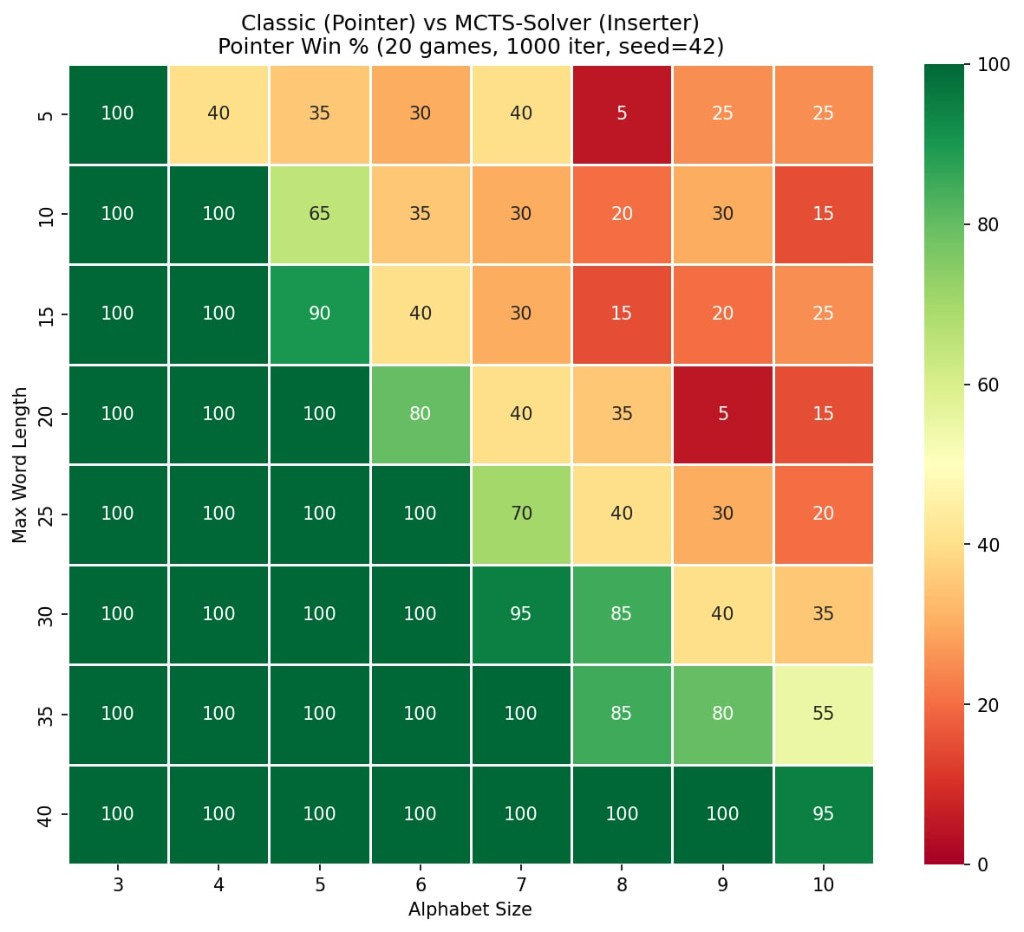
\includegraphics[width=0.75\textwidth]{figures/hm_classic_vs_solver.png}
\caption{Klasyczny UCT w roli Pointera przeciw MCTS-Solver w roli
Insertera -- wynik wyraźnie gorszy niż dla pozostałych wariantów.}
\label{fig:solver_inserter}
\end{figure}

Odwrócony układ ujawnia natomiast wyraźną regresję: MCTS-Solver w roli
Insertera przegrywa znacznie częściej niż jakikolwiek inny wariant.
W skrajnych warunkach faworyzujących Insertera (np.\ $L=5$, $|\Sigma|=10$)
zwycięża jedynie w $75\%$ partii, podczas gdy zarówno klasyczny UCT, jak
i UCB1-Tuned, w analogicznych konfiguracjach osiągają $100\%$. Łączny
zagregowany odsetek wygranych MCTS-Solver w obu rolach wynosi
$\approx 41{,}8\%$ (klasyczny UCT $\approx 58{,}2\%$); różnica
$\approx 16$ punktów procentowych jest istotnie większa niż jakakolwiek
zaobserwowana między pozostałymi wariantami.

Konfrontując wyniki z hipotezami:
\begin{itemize}
    \item \textbf{Hipoteza H2A okazuje się fałszywa.} MCTS-Solver
    \emph{nie} jest skuteczniejszy od klasycznego UCT; przeciwnie -- po
    uśrednieniu wyników w obu rolach \emph{przegrywa} z Classic
    o kilkanaście punktów procentowych.
    \item \textbf{Hipoteza H2B okazuje się prawdziwa, ale w mocniejszej
    formie.} Brak przewagi Solvera ujawnia się nie tylko ,,przy głębokim
    drzewie'', lecz w niemal całej badanej siatce, gdy gracz pełni rolę
    Insertera.
\end{itemize}

% --------------------------------------------------------------------------------------------
\section{Wnioski}

\subsection{Podsumowanie weryfikacji hipotez}

\begin{table}[H]
\centering
\begin{tabular}{>{\bfseries}l p{3.4cm} p{8cm}}
\toprule
Hipoteza & Wynik & Komentarz \\
\midrule
H1 & nie potwierdzona & UCB1-Tuned i klasyczny UCT osiągają w obu rolach
łącznie praktycznie identyczne wyniki ($\approx 49{,}8\%$ vs.\
$\approx 50{,}2\%$). \\
H2A & obalona & MCTS-Solver przegrywa z klasycznym UCT o kilkanaście
punktów procentowych w łącznym odsetku zwycięstw, głównie z powodu
regresji w roli Insertera. \\
H2B & potwierdzona, mocniejsza & Solver nie wykazuje przewagi nad
klasycznym UCT w żadnym fragmencie badanej siatki, niezależnie od
głębokości drzewa. \\
H3 & potwierdzona (silna) & Heurystyczna symulacja daje największą
poprawę spośród badanych modyfikacji ($\approx 64\%$ vs.\ $\approx 36\%$
dla klasycznego UCT). \\
H4 & potwierdzona & Wynik gry mocno determinuje stosunek
$L/|\Sigma|$; gradient widoczny we wszystkich heatmapach. \\
\bottomrule
\end{tabular}
\caption{Status weryfikacji postawionych hipotez.}
\end{table}

\subsection{Komentarz do regresji MCTS-Solver}

Wynik MCTS-Solver wymaga krótkiego komentarza, ponieważ jest sprzeczny
z teorią -- dodanie informacji o gwarantowanych wygranych i przegranych
nie powinno pogarszać jakości algorytmu. W naszym przypadku pogarsza
się ona głównie w roli Insertera, co wskazuje, że źródło problemu nie
leży w samej idei MCTS-Solver z literatury, lecz w tym, jak jego
elementy zostały spięte z resztą algorytmu w naszej implementacji.

Najbardziej prawdopodobnym mechanizmem regresji jest interakcja między
flagami udowodnionych węzłów a finalnym wyborem ruchu w korzeniu drzewa.
Klasyczny MCTS wybiera ruch o największej liczbie odwiedzin i to samo
kryterium zostało zachowane przy włączonym Solverze. Pozostawia to
otwartą furtkę: dziecko, które przed swoim udowodnieniem zdążyło zebrać
wiele wizyt (a potem zostało oznaczone jako proven loss i przestało być
rozwijane), może w finalnym podsumowaniu wciąż okazać się ,,najczęściej
odwiedzane''. W naszej grze taka sytuacja zdarza się nieproporcjonalnie
często właśnie po stronie Insertera, ponieważ proven loss bywa tu
udowadniany szybko, podczas gdy proven win wymagałby dotarcia symulacją
aż do limitu $L$. To tłumaczy zarówno asymetrię między rolami, jak
i charakter regresji.

Wydaje się więc, że obserwowane zachowanie należy zaliczyć do kategorii
problemów implementacyjnych -- konkretnie, do niedostatecznie spójnego
potraktowania udowodnionych etykiet na różnych etapach algorytmu --
a nie do wad samego MCTS-Solver jako modyfikacji.

\bibliographystyle{plain}
\bibliography{lit}

\end{document}
